\documentclass[a4paper, 11pt]{article}

\usepackage{enumitem}
\usepackage{graphicx}
\usepackage{hyperref}
\usepackage[utf8]{inputenc}
\usepackage{minted}

\begin{document}

\title{
	\textbf{Sorting an Array in C}
}
\author{Neo Gullberg}
\date{Fall 2024}
\maketitle

\section{Introduction}
	In this assignment my task was to implement and benchmark some sorting algorithms in C, namely:
	\textit{selection sort}, \textit{insertion sort}, and \textit{merge sort}.
	Similar to prior assignments we also needed to try and find the time complexity for each algorithm,
	which I thought was somewhat harder this time around (but more on that later).

\section{Selection Sort}
	The first one on the list was selection sort.
	Selection sort begins at the start of the array and goes through every index (except the last one).
	For each index it loops through each index ahead and looks for the minimum value amongst them.
	If a minimum value is found, that value is swapped with the value of the current index.
	Then it continues to the next index and repeats the process until the last element.
	The last element doesn't need to be processed since all prior iterations will have made sure that this element is of the highest value present in the array.
	\begin{figure}[H]
		\centering
		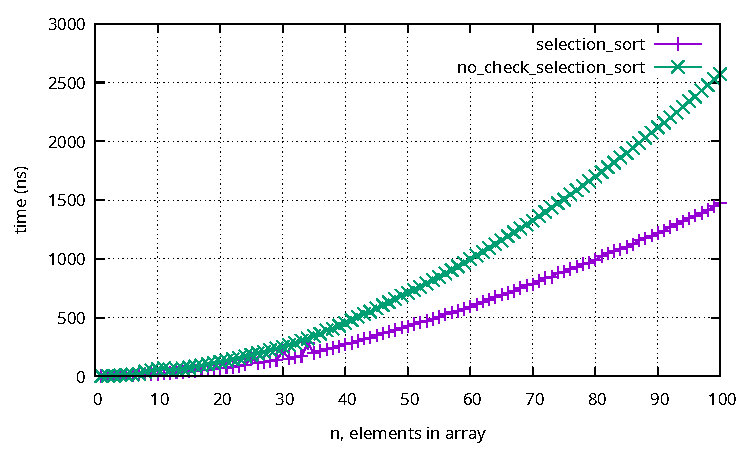
\includegraphics[scale=0.7]{graphs/selection_sort_vs_no_check_selection_sort.pdf}
		\caption{
			Graph showing the time it took to sort an array with selection sort.
		}
	\end{figure}
	In the \textbf{Figure 1} we see that the time complexity for selection sort seems to be \(O(n^2)\).
	You probably noticed that there are two lines in the graph.
	I was interested in seeing how much of a performance benefit (if any at all) comes from the check to see if a minimum value has indeed been found,
	opposed to always performing a swap.
	I thought that it might have been faster to always swap, instead of always checking.
	So I ran a benchmark, but as can be seen in the result it seems I was quite wrong.

\section{Insertion Sort}
	Up next was insertion sort.
	Similar to selection sort, insertion sort also loops through every index from start to finish (this time including the last entry, but skipping the first).
	Where it differs is how each index is handled.
	For each index it starts going backwards.
	If it ever finds a value that is bigger than itself they swap places, and continues to traverse backwards until it meets an element smaller than itself.
	Since we've already sorted the prior elements we know that no bigger elements exist beyond that point.
	\begin{figure}[H]
		\centering
		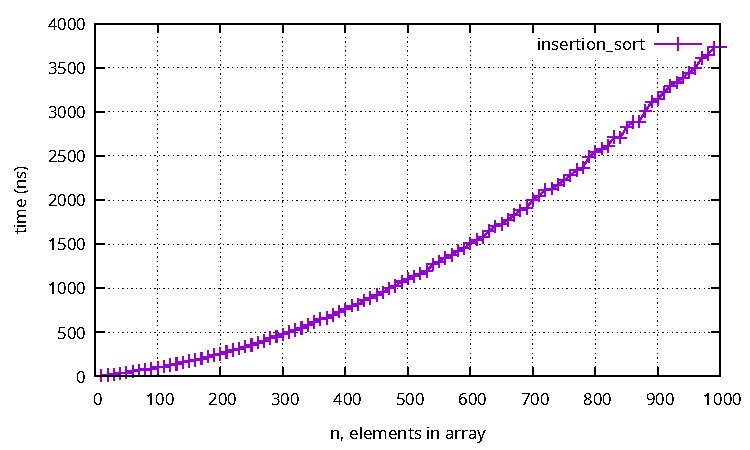
\includegraphics[scale=0.7]{graphs/insertion_sort.pdf}
		\caption{
			Graph showing the time it took to sort an array with insertion sort.
		}
	\end{figure}
	In \textbf{Figure 1} we saw that selection sort took around 1500 ns to sort 100 elements,
	whilst \textbf{Figure 2} shows that insertion sort could sort around 600 elements in the same time.
	This clearly shows that selection sort is faster than insertion sort.
	The difference mainly comes from selection sort having to loop through all of the unsorted elements each outer iteration,
	whilst insertion sort loops through the sorted part which will generally be faster.
	So far all measurements have been carried out on arrays with random values.
	However, what if the array was sorted to begin with?
	\begin{figure}[H]
		\centering
		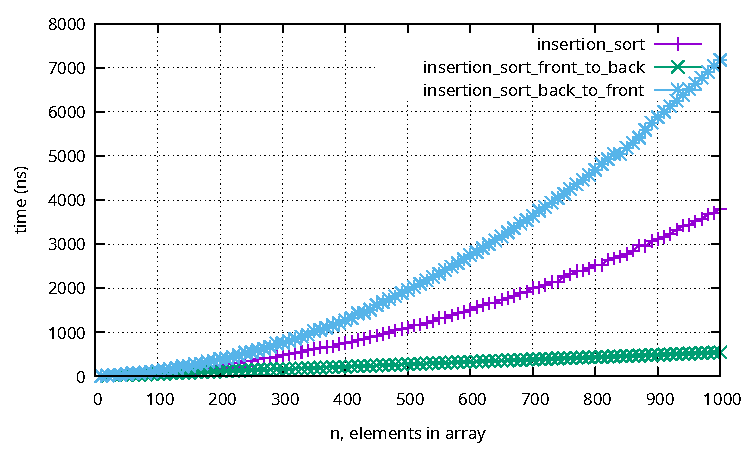
\includegraphics[scale=0.7]{graphs/insertion_sort_vs_insertion_sort_front_to_back_vs_insertion_sort_back_to_front.pdf}
		\caption{
			Graph comparing insertion sort on different kinds of arrays.
		}
	\end{figure}
	\textbf{Figure 3} shows that it takes almost double as long for insertion sort when the array is sorted back to front.
	But when the opposite is true the time it takes is much faster.
	When it is sorted front to back the time complexity is actually \(O(n)\) since each backwards check ends immediately and therefore
	the time it takes grows linearly with the size of the array.

\section{Merge Sort}
	Last was merge sort.
	Merge sort works by dividing the array into halfs over and over again with recursion until we're only left with individual elements,
	then from those we begin sorting and \textit{merging} them back together following the order they were split.
	We build our way up to larger and large segments untill we are left with the whole array sorted.
	The nice thing about doing it this way is that the merges will always be done on arrays that are themselves sorted which means
	the merging can be done very fast.
	If we wanted to merge two sorted arrays, A and B, it would work something like this:
	\begin{itemize}[label=\textbullet]
		\item If A is empty, choose the first element from B.
		\item If B is empty, choose the first element from A.
		\item If both contain at least one element, we compare the first element of each and pick the one that is smaller.
	\end{itemize}
	When an element is taken it is of course added to the correct place in the original array, and removed from from where it was taken.
	This is how I think about it, but the way I implemented it in code is technically a bit different.
	\par
	To avoid the need of having to allocate memory for two new arrays each split we can instead allocate one array, as big as the array we want sorted,
	before any splitting or merging is done.
	\begin{minted}[obeytabs=true, tabsize=4]{c}
void merge_sort_merge(int *array, int *tmp, size_t lo, size_t mid, size_t hi)
{
	for (size_t i = lo; i <= hi; i++) tmp[i] = array[i];

	size_t left_half_start = lo;
	size_t right_half_start = mid + 1;
	for (size_t i = lo; i <= hi; i++)
	{
		if (left_half_start > mid)
			array[i] = tmp[right_half_start++];
		else if (right_half_start > hi)
			array[i] = tmp[left_half_start++];
		else if (tmp[left_half_start] < tmp[right_half_start])
			array[i] = tmp[left_half_start++];
		else
			array[i] = tmp[right_half_start++];
	}
}
	\end{minted}
	The code I wrote starts by copying the values we want sorted into the extra array I mentioned which I called \texttt{tmp}.
	It is important to have the elements we want to sort stored separetely from where we want them to be sorted.
	If we would not separate them it would in most cases result in the merge algorithm sorting elements that have already been sorted.
	The for loop loops from a lower-bound \texttt{lo} to an upper-bound \texttt{hi} which define the size of the segment to be merged.
	\texttt{mid} denotes the separation between the "arrays" to be merged (they are actually just parts of one larger array).
	The variables \texttt{left\_half\_start} and \texttt{right\_half\_start} keep track of were the arrays start,
	which gets incremented whenever an element is "removed" from the respective side.
	The first if check represents checking if the left half is empty, and will then pick from the right half.
	The second if check does the same but reversed.
	The last two cases represents when both arrays contain atleast one element, and picking the element that is smallest.
	\begin{figure}[H]
		\centering
		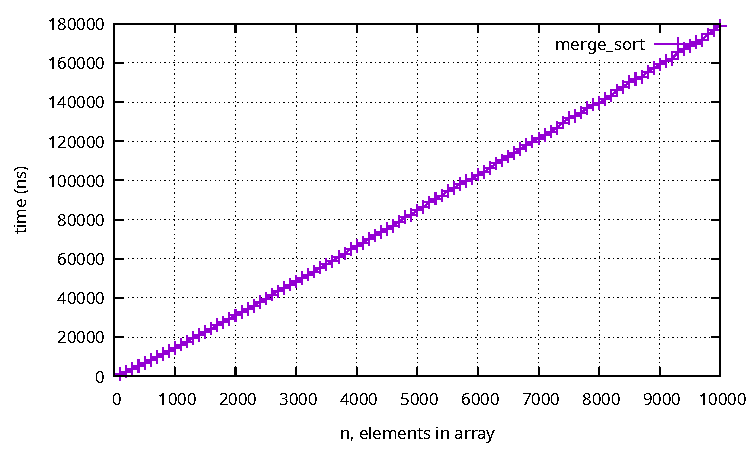
\includegraphics[scale=0.7]{graphs/merge_sort.pdf}
		\caption{
			Graph showing the time it took to sort an array with merge sort.
		}
	\end{figure}
	\textbf{Figure 4} shows my measurements for merge sort.
	At first it looks eerily similar to a time complexity of \(O(n)\).
	That means our graph should turn roughly \(O(1)\) if we divide every measurement with the number of elements at that time. So let's try it!
	\begin{figure}[H]
		\centering
		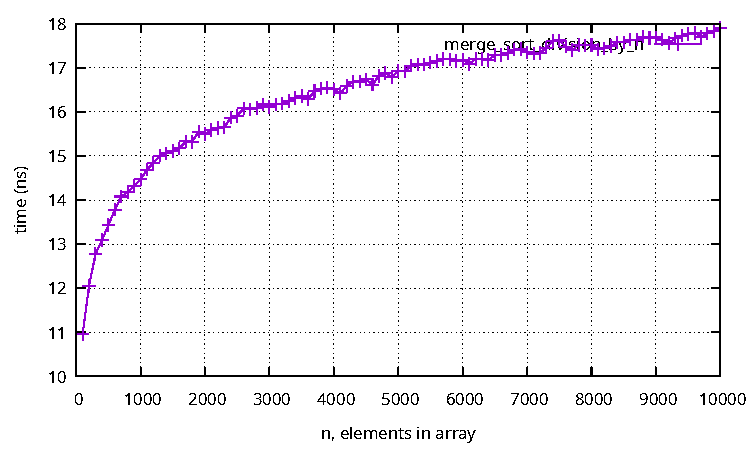
\includegraphics[scale=0.7]{graphs/merge_sort_division_by_n.pdf}
		\caption{
			Graph showing the time it took to sort an array with merge sort, where each measurement is divided by \(n\).
		}
	\end{figure}
	\textbf{Figure 5} looks similar to \(O(\log n)\) which would suggest that the time complexity of our merge sort is actually \(n \cdot O(\log n)\)
	(by multiplying with the \(n\) we just divided by).
	This is what I thought was a bit harder to find compared to earlier assignments.
	At first I was a fool and thought that merge sort actually had a time complexity of \(O(n)\), but it is easy to make that mistake at first glance.
	\begin{figure}[H]
		\centering
		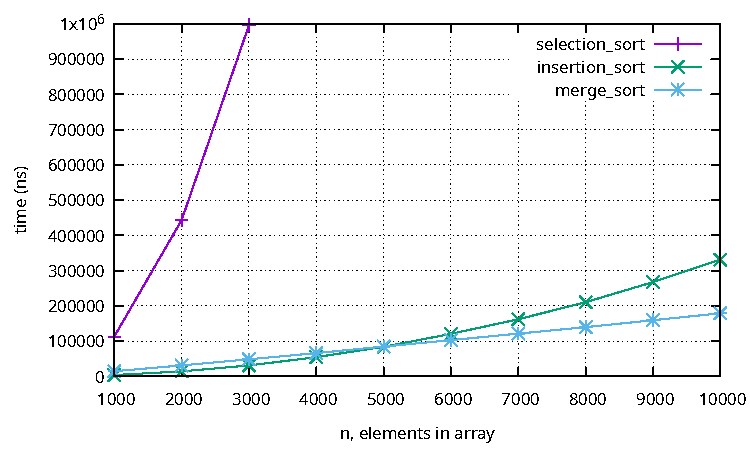
\includegraphics[scale=0.7]{graphs/selection_sort_vs_insertion_sort_vs_merge_sort.pdf}
		\caption{
			Graph comparing all the sorting algorithms gone through in this assignment.
		}
	\end{figure}
	At last \textbf{Figure 6} displays a comparison between the three sorting algorithms we've talked about.
	We see that selection sort is by far the worst performing one out of the lot.
	And expectedly merge sort performs best in the long run which we could guess from its less severe time complexity.
	However, it is interesting to note that insertion sort looks to be faster up until around 5000 mark,
	which means it would actually be preferred over merge sort for many use cases that don't have the need to sort very large datasets.

\section{Source Code}
	If anyone is interested, the source code for this project can be found over at:
	\url{https://github.com/neogulgul/ID1021/tree/main/sorting}

\end{document}
